% Copyright 2004 by Till Tantau <tantau@users.sourceforge.net>.
%
% In principle, this file can be redistributed and/or modified under
% the terms of the GNU Public License, version 2.
%
% However, this file is supposed to be a template to be modified
% for your own needs. For this reason, if you use this file as a
% template and not specifically distribute it as part of a another
% package/program, I grant the extra permission to freely copy and
% modify this file as you see fit and even to delete this copyright
% notice. 

\documentclass[tikz]{beamer}

\setbeamertemplate{caption}[numbered]
\setbeamercovered{invisible}
\usepackage{mwe,tikz}
\usepackage{gensymb}
\usepackage[percent]{overpic}
\usepackage{animate}
\usepackage{bm}
\usepackage{amsmath}
% \usepackage{onimage}
% There are many different themes available for Beamer. A comprehensive
% list with examples is given here:
% http://deic.uab.es/~iblanes/beamer_gallery/index_by_theme.html
% You can uncomment the themes below if you would like to use a different
% one:
% \usetheme{AnnArbor}
% \usetheme{Antibes}
% \usetheme{Bergen}
% \usetheme{Berkeley}
% \usetheme{Berlin}
\usetheme{Boadilla}
% \usetheme{boxes}
% \usetheme{CambridgeUS}
% \usetheme{Copenhagen}
% \usetheme{Darmstadt}
% \usetheme{default}
% \usetheme{Frankfurt}
% \usetheme{Goettingen}
% \usetheme{Hannover}
% \usetheme{Ilmenau}
% \usetheme{JuanLesPins}
% \usetheme{Luebeck}
% \usetheme{Madrid}
% \usetheme{Malmoe}
% \usetheme{Marburg}
% \usetheme{Montpellier}
% \usetheme{PaloAlto}
% \usetheme{Pittsburgh}
% \usetheme{Rochester}
% \usetheme{Singapore}
% \usetheme{Szeged}
% \usetheme{Warsaw}
\usetikzlibrary{arrows,decorations.markings,decorations.pathmorphing, patterns,shapes}

\title{The Double Pendulum}

% A subtitle is optional and this may be deleted
\subtitle{Creating the Perfect Baseball Bat}

\author{Jared Baur}
% - Give the names in the same order as the appear in the paper.
% - Use the \inst{?} command only if the authors have different
%   affiliation.

\institute[Occidental College] % (optional, but mostly needed)
{
  Physics Department\\
  Occidental College
% - Use the \inst command only if there are several affiliations.
% - Keep it simple, no one is interested in your street address.
}
\date{February 25, 2019}
% - Either use conference name or its abbreviation.
% - Not really informative to the audience, more for people (including
%   yourself) who are reading the slides online

% \subject{Theoretical Computer Science}
% % This is only inserted into the PDF information catalog. Can be left
% % out. 

% % If you have a file called "university-logo-filename.xxx", where xxx
% % is a graphic format that can be processed by latex or pdflatex,
% % resp., then you can add a logo as follows:

% % \pgfdeclareimage[height=0.5cm]{university-logo}{university-logo-filename}
% % \logo{\pgfuseimage{university-logo}}

% Delete this, if you do not want the table of contents to pop up at
% the beginning of each subsection:

% \AtBeginSubsection[]
% {
%   \begin{frame}<beamer>{Outline}
%     \tableofcontents[currentsection,currentsubsection]
%   \end{frame}
% }

% Let's get started
\begin{document}

\begin{frame}
  \titlepage
\end{frame}

\begin{frame}{Scope}
  \tableofcontents
  % You might wish to add the option [pausesections]
\end{frame}

% Section and subsections will appear in the presentation overview
% and table of contents.

\section{Introduction}

\begin{frame}{The Double Pendulum}
	\only<1> {	
    		\begin{figure}
		    \centering
		    \animategraphics[loop,controls,width=\linewidth,scale=0.6]{10}{doublependulum_gif/doublependulum-}{0}{297}
		\end{figure}
	}
	\only<2> {
    		\begin{figure}
		    \centering
		    \animategraphics[loop,controls,width=\linewidth,scale=0.6]{10}{comparison_gif/comparison-}{0}{99}
		\end{figure}

		Chaos increases exponentially
		\begin{equation}
			\Delta x(t) \sim \Delta x(t_0) e^{\lambda t}
		\end{equation}
	}
	\only<3> {
		Chaos is not as prevalent in a baseball swing, due to the swing only occuring in the first half cycle of a double pendulum
    		\begin{figure}
		    \centering
		    \animategraphics[loop,controls,width=\linewidth,scale=0.6]{10}{baseballswing_gif/baseballswing-}{0}{23}
		\end{figure}
		Can we design a ``perfect" baseball bat?
	}
	% \only<4> {
	% 	Can we design a "perfect" baseball bat?
	% }
\end{frame}

\section{Equations of Motion}

\begin{frame} {Equations of Motion}

	\only<1> {
		\begin{figure}
			\centering
			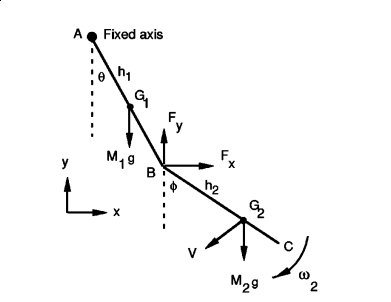
\includegraphics[scale=0.75]{equationsofmotion.png}
		\end{figure}
	}
	
	\only<2> {
		Coordinates $(x,y)$ of $G_2$, with respect to origin $A$:
		\begin{equation}
			L_1 \sin{\theta} + h_2 \sin{\phi} - L_1 \cos{\theta} - h_2 \sin{\phi} \tag{1}
		\end{equation}
		
		With $V$ as the velocity of $G_2$, components of $V$ are given as:
		\begin{equation}
			V_x = \frac{dx}{dt} = -L_1 \omega_1 \cos{\theta} - h_2 \omega_2 \cos{\phi} \tag{2}
		\end{equation}
		\begin{equation}
			V_y = \frac{dy}{dt} = -L_1 \omega_1 \sin{\theta} - h_2 \omega_2 \sin{\phi} \tag{3}
		\end{equation}
	}

	\only<3> {
		Forces arm exerts on rod:
		\begin{equation*}
			\begin{aligned}
				F_x & = M_2 \frac{d V_x}{dt} \\
				    & = -M_2 \bigg [ L_1 \cos{\theta} \frac{d \omega_1}{dt} + L_1 \omega_1^2 \sin{\theta} + h_2 \cos{\phi} \frac{d \omega_2}{dt} + h_2 \omega_2^2 \sin{\phi} \bigg ]
			\end{aligned}
		\end{equation*}

		\begin{equation*}
			\begin{aligned}
				F_y - M_2 g & = M_2 \frac{d V_y}{dt}\\
				 % & = \\
				& = -M_2 \bigg [ L_1 \sin{\theta} \frac{d \omega_1}{dt} - L_1 \omega_1^2 \cos{\theta} + h_2 \sin{\phi} \frac{d \omega_2}{dt} - h_2 \omega_2^2 \cos{\phi} \bigg ]
			\end{aligned}
		\end{equation*}
	}

	\only<4> {
		Torque from muscles, $C_1$ is applied on arm and $C_2$ is applied on the rod. The arm applies an equal and opposite torque $-C_2$ to the rod. \\
		Initial conditions: $\theta = 90\degree$, $\phi = 180\degree$, and $\beta = \theta - \phi = 90\degree$.

		\begin{figure}
			\centering
			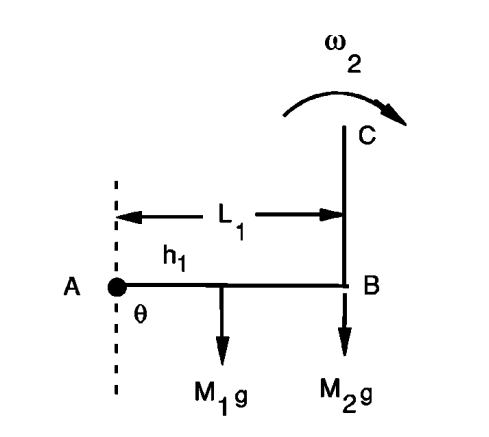
\includegraphics[scale=0.4]{wristcock.png}
		\end{figure}
	}

	\only<5> {
		When $C_1$ and $C_2$ equal zero, initial angular accelerations are
		\begin{equation}
			\frac{d \omega_1}{dt} = (M_1 h_1 + M_2 L_1)g/A \tag{6}
		\end{equation}

		\begin{equation}
			\frac{d \omega_2}{dt} = 0 \tag{7}
		\end{equation}

		Rod acts as point mass at the end of the arm since it has no initial angular acceleration, so the total moment of inertia of the arm and rod is
		\begin{equation}
			I_1 +M_2 L_2^2 = A
		\end{equation}

	}

	\only<6> {
		In practice, initial stage of swing is in "wrist-cock" position. After arm has rotated to about $\theta = 45 \degree$, torque from centripetal force is large enough to swing the rod without assistance from the wrist.
		\begin{figure}
			\centering
			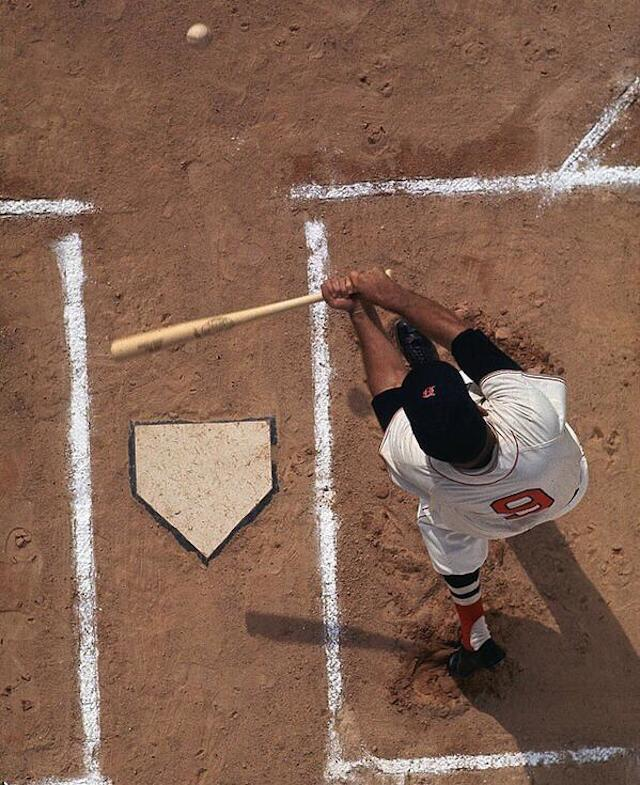
\includegraphics[scale=0.2]{aerialswing.jpg}
		\end{figure}
	}

\end{frame}


\section{Experimental Results}
\begin{frame} {Experimental Results}
	
	\only<1> {
		With the spot mechanism, $\beta$ cannot exceed $90 \degree$ and the pendulum initially rotates as a rigid body
		\begin{figure}
			\centering
			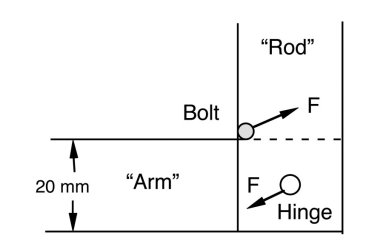
\includegraphics[scale=0.5]{stopmechanism.png}
		\end{figure}
	}

	\only<2> {
		Chaotic motion is highly dependent on the initial conditions of the arm and rod, however this chaos develops mostly after the first half cycle of motion.
		\begin{figure}
			\centering
			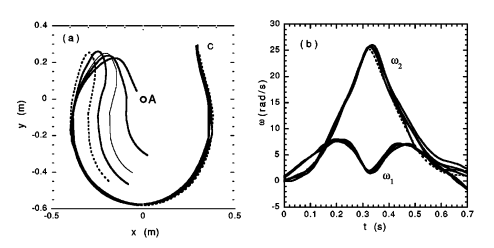
\includegraphics[scale=0.5]{trajectory.png}
		\end{figure}

		The area of interest with the double pendulum swing is the point where the lower segment of the rod reaches its maximum speed and shortly afterward.
	}

	\only<3> {
		\begin{figure}
			\centering
			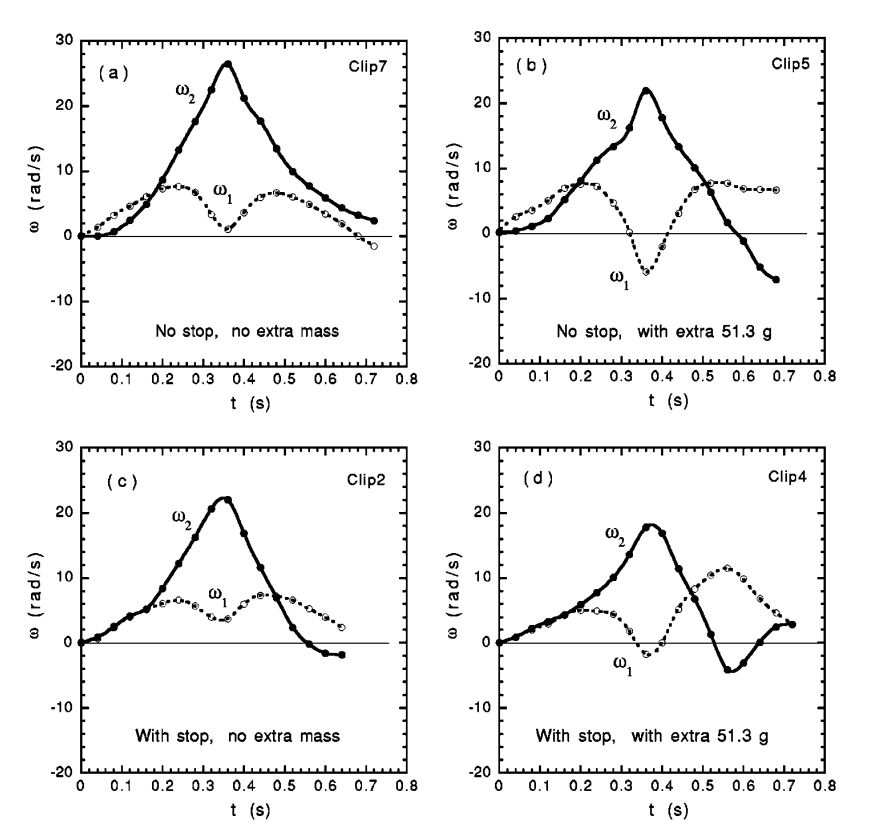
\includegraphics[scale=0.25]{angularvelocities.png}
		\end{figure}
	}

	\only<4> {
		Observations:\\
		\begin{itemize}
			\item $\omega_1 = \omega_2$ for first 0.2 seconds with stop
			\item Angular speed of arm is at minimum when angular speed of rod is at maximum
		\end{itemize}

		\begin{figure}
			\centering
			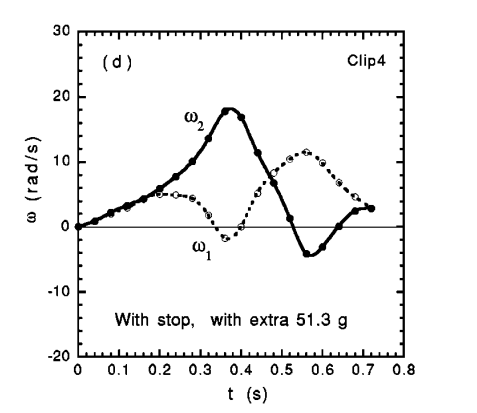
\includegraphics[scale=0.35]{angularvelocityrealistic.png}
		\end{figure}
	}

\end{frame}

\section{Energy Transfer}

\section{Applications}

% \section*{Resources}
\end{document}

